\chapter{Introduction}

The adoption of container-based architectures and orchestrators such as Kubernetes has transformed how applications are developed and deployed in cloud and enterprise environments. This paradigm enables automated lifecycle management of applications, improves scalability and facilitates the integration of modern development practices. However, this technological evolution also introduces new security challenges, especially in environments where deployments are carried out in an automated and continuous manner.

In this context, the DevSecOps approach has emerged, with the objective of integrating security within the software development lifecycle itself, rather than treating it as a post-deployment phase. This model promotes the automation of security controls within continuous integration and deployment pipelines, enabling the detection of vulnerabilities, the application of security policies and the guarantee of secure configurations from the earliest stages of development.

This Master's Thesis focuses on the implementation of a complete DevSecOps environment on Kubernetes, integrating Continuous Integration tools (GitHub Actions) with automated vulnerability analysis using tools such as Trivy and Sysdig Secure. A GitOps-based Continuous Deployment model using ArgoCD is also implemented, enabling the declarative management of infrastructure and deployments through Git repositories.

Additionally, Kyverno is incorporated as a Policy-as-Code security policy engine, enabling the automatic enforcement of controls over Kubernetes manifests during the deployment process.

The core of the project is based on the use of Admission Controllers, specifically Kyverno, to apply security policies declaratively within the Kubernetes cluster. Unlike traditional approaches that only block insecure configurations, this work explores the use of mutating policies, capable of automatically correcting insecure configurations in YAML manifests at deployment time.

Finally, the project includes a comparative analysis between Kyverno and OPA Gatekeeper, evaluating their capabilities in implementing security policies in Kubernetes, their ease of use, learning curve and effectiveness in production environments.

Figure~\ref{fig:arquitectura-devsecops} shows a general overview of the DevSecOps architecture implemented in this work, where development processes, security analysis, continuous deployment and policy enforcement are all integrated within a Kubernetes environment.

\begin{figure}[H]
\centering
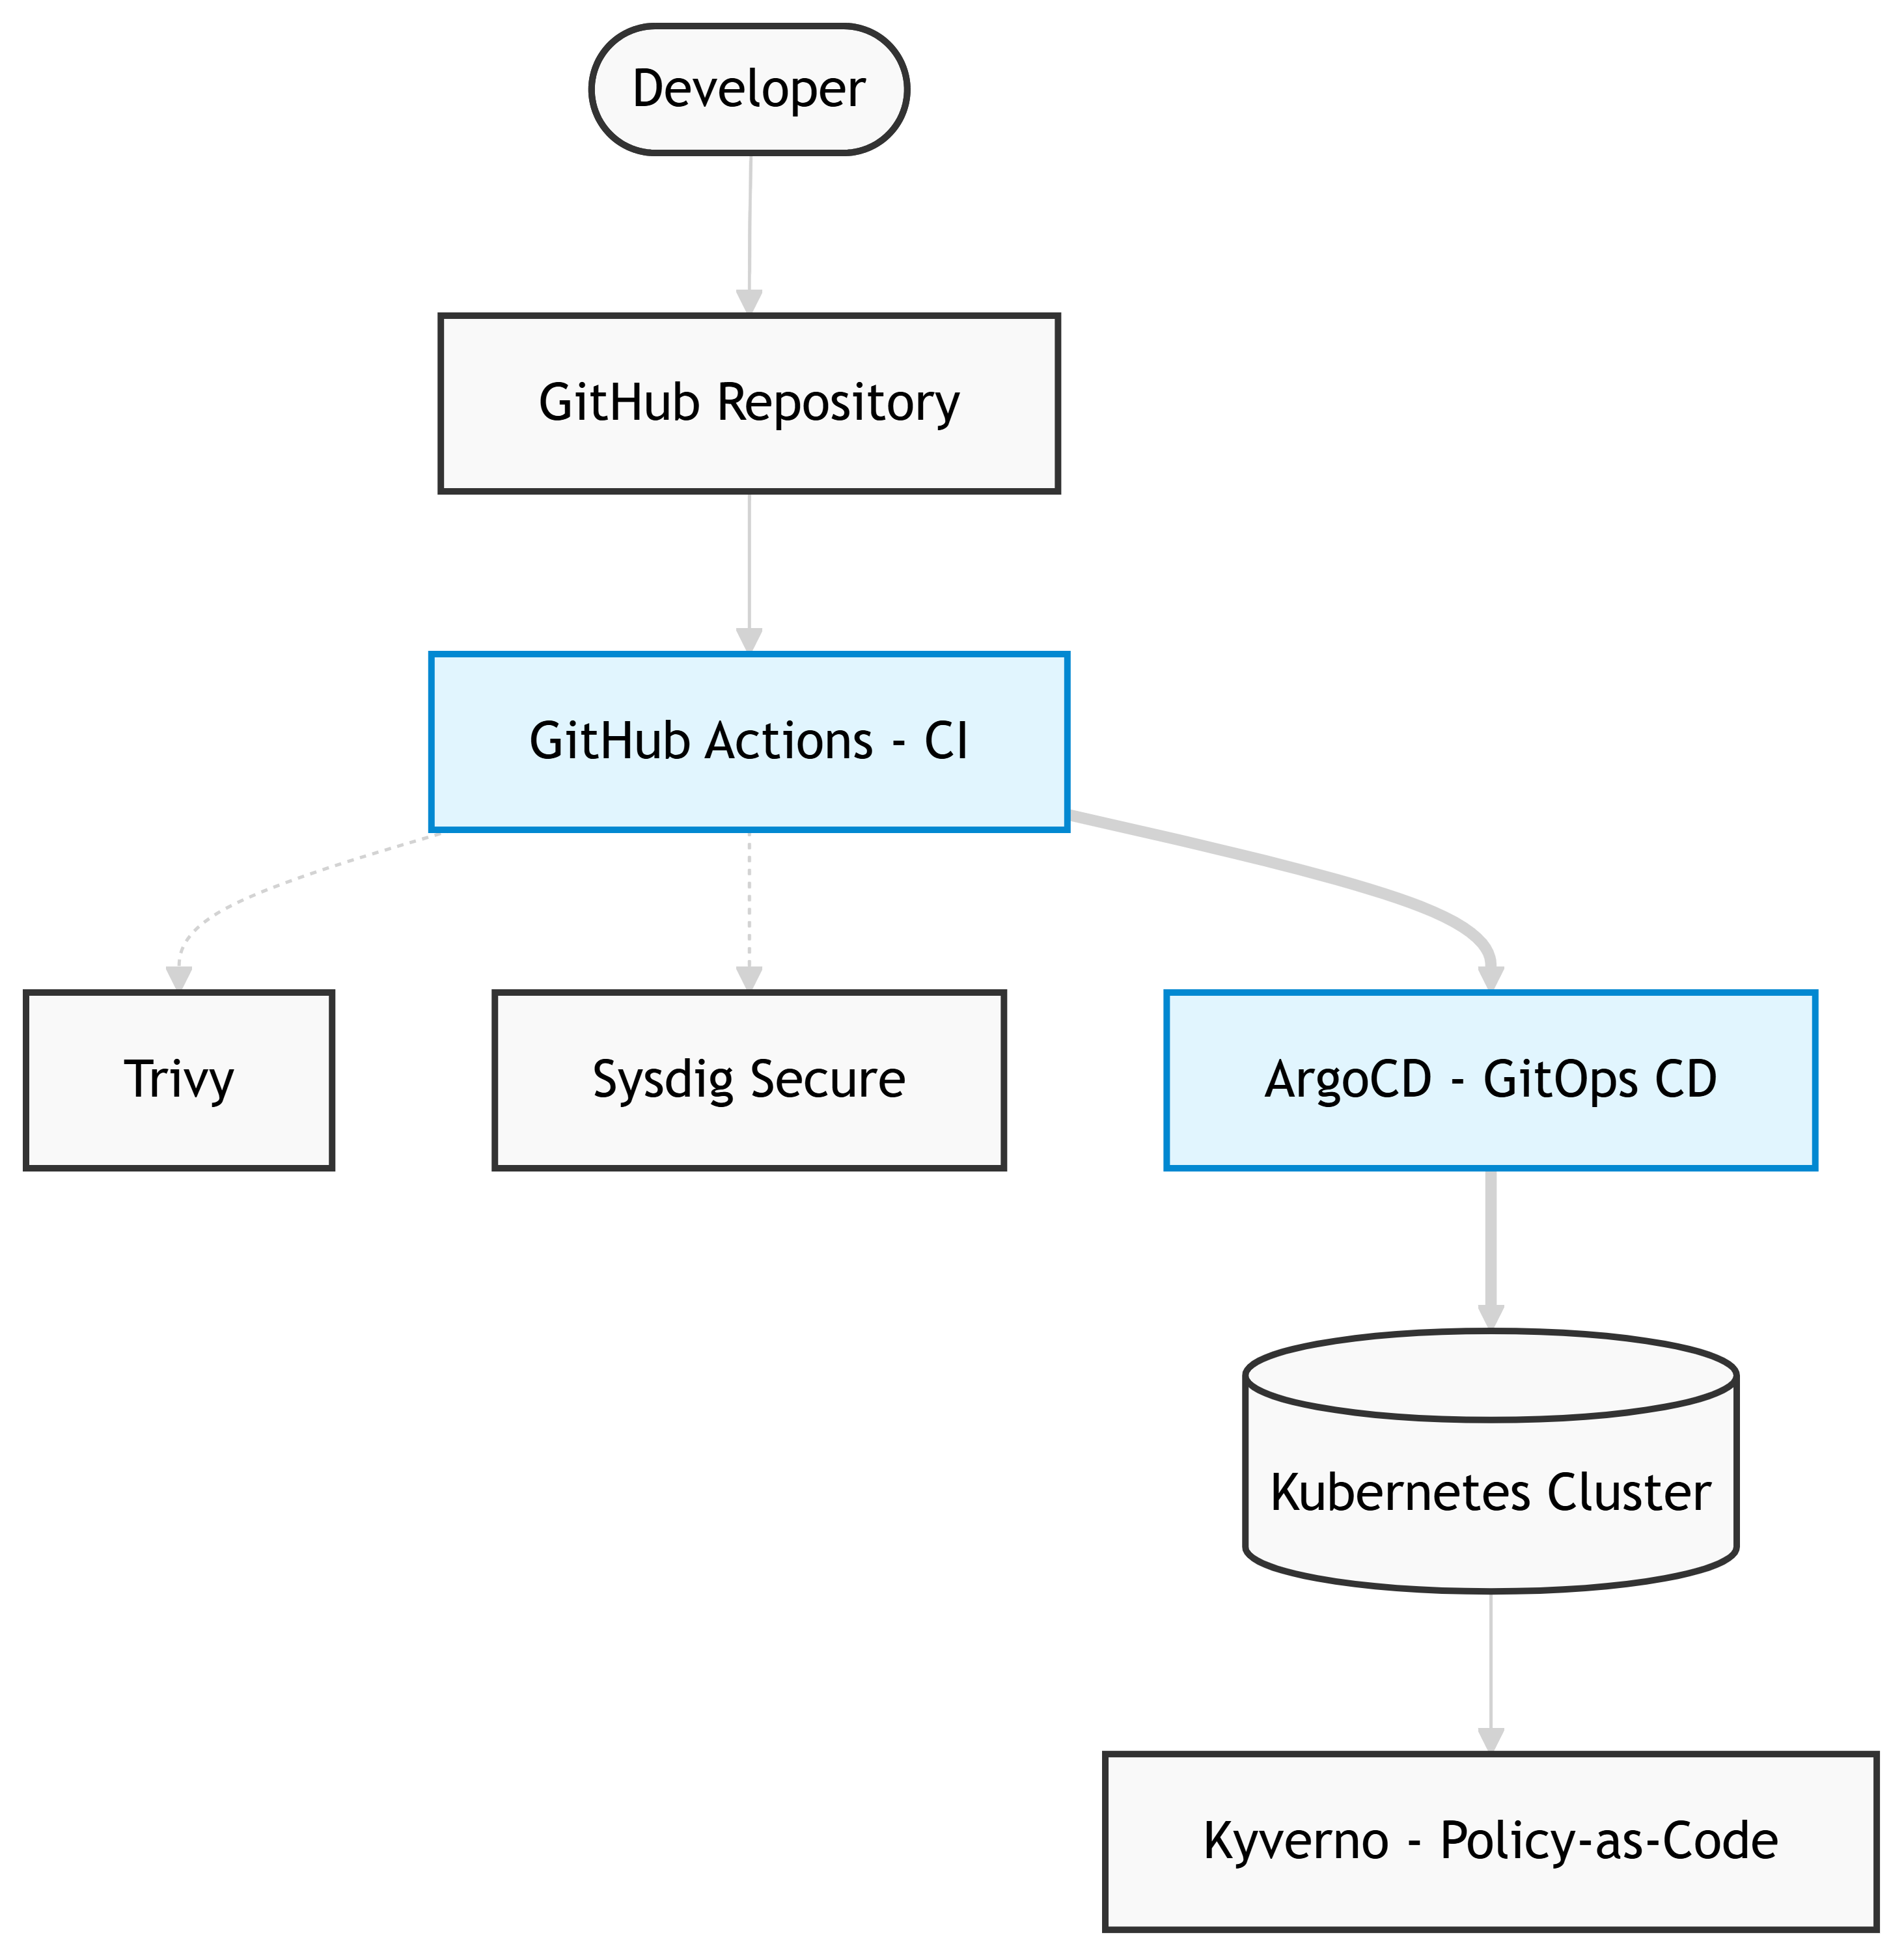
\includegraphics[width=0.5\linewidth]{images/arquitectura_DevSecOps.png}
\caption{General architecture of the DevSecOps environment}
\label{fig:arquitectura-devsecops}
\end{figure}
